\chapter{Kajian Literatur}\label{c2}%

\section{Pengenalan}
Kajian literatur merupakan suatu kajian terhadap keperluan pembangunan projek. Semasa kajian ini dilakukan, segala maklumat-maklumat berkaitan telah dikumpulkan bagi memahami dan mengenalpasti masalah-masalah yang terlibat, kekangan-kekangan dalam pembangunan, teknologi perkakasan dan perisian yang sesuai, dan lain-lain lagi. Kaedah kajian literatur perlu dilakukan dengan teliti kerana ianya adalah amat penting untuk merangka
perancangan penyelesaian bijak bagi menjamin kelancaran pelaksanaan kajian dan seterusnya menjamin keberkesanan aplikasi yang bakal dibangunkan kerana kegagalan mengenalpasti masalah-masalah yang berkaitan semasa peringkat kajian literatur ini boleh membawa kepada kegagalan kajian secara keseluruhannya.

\section{Kajian Kepada Antaramuka Sistem Terbenam Linux}
Antaramuka sedia ada dalam sistem terbenam Linux Realtime Rain Gauge terhad kepada penggunaan Antaramuka Baris Perintah atau lebih dikenali sebagai CLI sebagai singkatan kepada \textit{Command Line Interface}. Ini bagi meminimakan penggunaan sumber di dalam sistem yang padat dan kecil. Antaramuka CLI telah digunakan bagi melakukan konfigurasi dan penyeliaan sistem terbenam ini hingga sekarang.

CLI telah diperkenalkan pada awal 1960-an. Sistem yang mula-mula menggunakan antaramuka baris perintah adalah sebuah mesin taip yang dikenali sebagai Tele-type (TTY). Seterusnya, CLI digunakan sebagai mekanisma interaksi sistem operasi dengan menaip arahan untuk menjalankan sesuatu tugas. Dalam antaramuka baris perintah, pengguna berinteraksi dengan sistem dengan cara menaip perintah secara baris demi baris. Antaramuka ini sedia berinteraksi dengan pengguna dengan menggunakan perintah-perintah yang berbentuk dialog soal-jawab.

Pada hari ini, antaramuka CLI ini telah jarang digunakan oleh pengguna komputer biasa. Pengguna biasa lebih selesa menggunakan antaramuka bergrafik yang lebih banyak menggunakan tetikus sebagai peranti arahan dengan cara mengetik butang tetikus pada ikon atau butang untuk melakukan sesuatu arahan. Namun begitu, penggunaan CLI masih popular dikalangan pengguna sistem operasi Linux dan Pentadbir Sistem untuk berkomunikasi dengan Pelayan.

Sistem terbenam linux umumnya tidak mempunyai antaramuka bergrafik bagi memastikan saiz sistem yang kecil dan optimum. Walau bagaimanapun, antaramuka bergrafik boleh ditambah pada sistem terbenam linux ini mengikut keupayaan sistem dan peranti yang ada pada sistem terbenam tersebut.

\subsection{Kajian Sistem dan Aplikasi Semasa}
Kaedah semasa untuk membuat konfigurasi dan penyelenggaraan bagi sistem terbenam Linux ialah menggunakan CLI. Pengguna perlu mempunyai pengetahuan asas dalam penggunaan sistem operasi Linux sekurang-kurangnya kerana mereka dikehendaki mengingat baris perintah yang perlu ditulis untuk melakukan sesuatu tugas. Terdapat dua cara untuk melakukan konfigurasi menggunakan CLI. Cara yang pertama ialah menggunakan sambungan RS-232 kepada port komunikasi perkakasan ini. Bagi pengguna Microsoft Windows, ia biasanya dipanggil COM port, manakala bagi pengguna Linux, ia dipanggil /dev/tty. Cara yang kedua pula menggunakan sambungan rangkaian dimana komputer boleh disambungkan secara terus menggunakan kabel rangkaian Cat-5 kepada perkakasan ini, melalui switch, hub, ataupun router. Command Line interface boleh diakses menggunakan SSH atau Telnet melalui sambungan rangkaian.

\begin{figure}[!h]
\centering{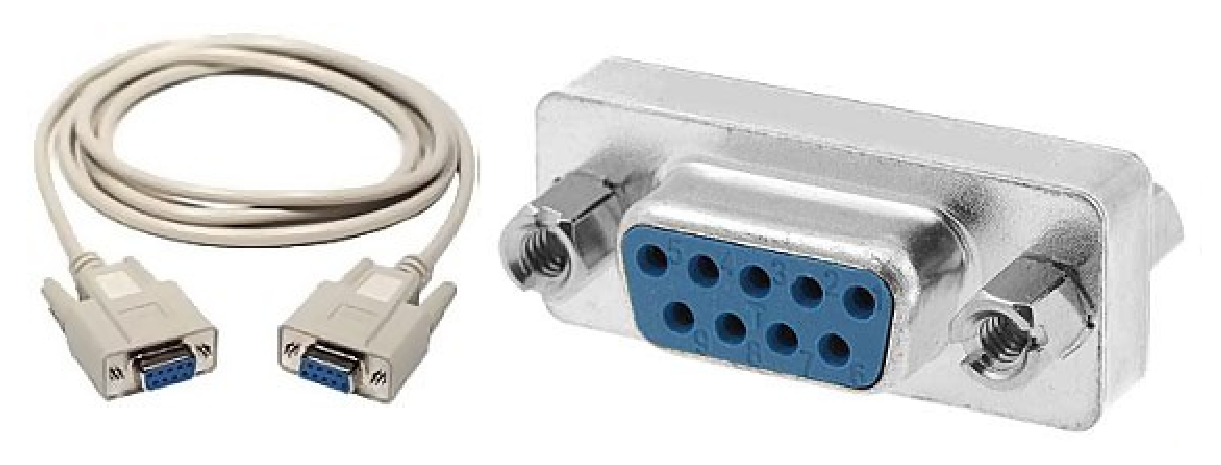
\includegraphics[width=0.9\textwidth]{source/fig/serial-cable.eps}}
\caption[Kabel Serial RS-232]{Kabel Serial RS-232}
\label{c2:f1}
\end{figure}

Bagi Sistem Terbenam Linux ini, Port /dev/tty yang boleh digunakan untuk terminal serial ialah /dev/ttyAM0 dan /dev/ttyAM1. Ia dipanggil /dev/ttyAM kerana perkakasan ini menggunakan pemandu serial jenis PORT\_AMBA. Untuk menyambungkan komputer melalui sambungan serial, kabel serial 9 pin dengan penyambung DB9 boleh disambungkan kepada port /dev/ttyAM0 perkakasan ini. Biasanya setiap komputer juga mempunyai satu port yang serupa, oleh itu satu kabel serial dengan kedua-dua bahagian penyambung DB9 Female boleh digunakan. 

Bagi komputer yang tidak mempunyai Port ini, Port USB boleh digunakan. Namun, ia memerlukan Converter yang dipanggil USB to Serial Converter. Converter ini boleh didapati di mana-mana kedai komputer dengan mudah. Setelah menyambungkan komputer kepada Sistem Terbenam Linux ini menggunakan kabel serial tersebut, Terminal Konsol Serial yang juga Command Line Interface boleh diakses menggunakan aplikasi Minicom dari sistem pengoperasian Linux atau Hyper Terminal dari sistem pengoperasian Windows.

\begin{figure}[!h]
\centering{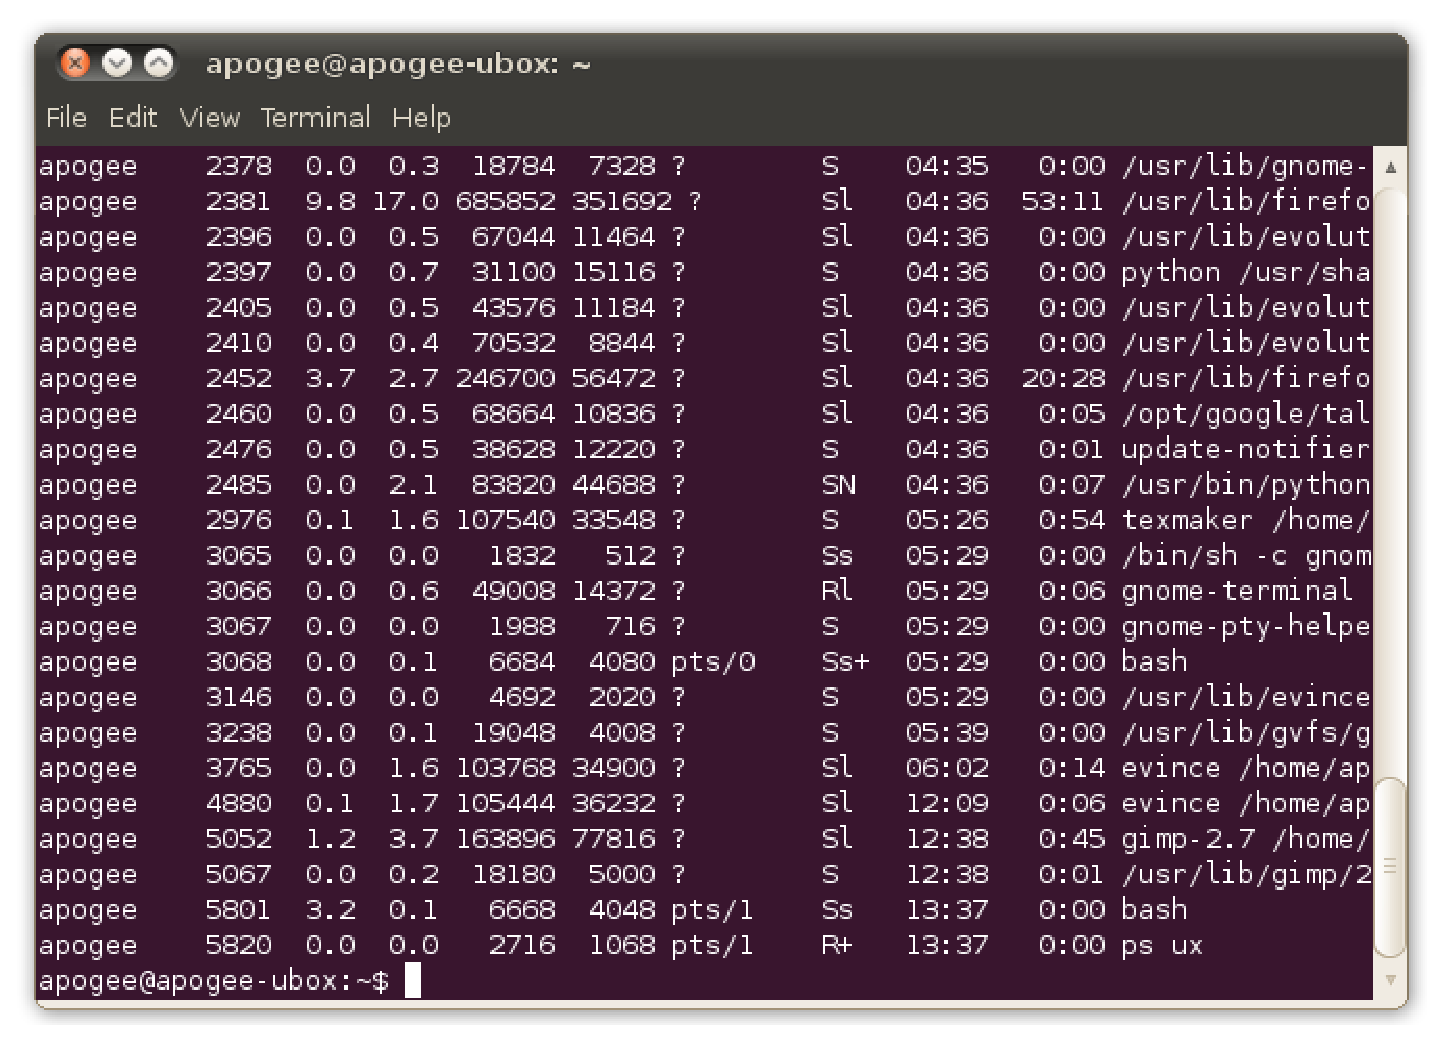
\includegraphics[width=0.9\textwidth]{source/fig/terminal-console.eps}}
\caption[Contoh paparan antaramuka CLI]{Contoh paparan antaramuka CLI yang kurang mesra pengguna}
\label{c2:f2}
\end{figure}

Daripada Terminal Konsol Serial ini, pengguna boleh berinteraksi dengan Sistem Terbenam Linux sepertimana mereka berinteraksi dengan Command Line Interface bagi sistem pengoperasian Linux yang lain. Dari sini, pengguna boleh mengubah, menambah dan memadam fail yang terdapat dalam sistem ini bagi menepati keperluan konfigurasi sistem. Namun, pengetahuan mengenai sistem pengoperasian Linux amat diperlukan kerana dengan kesilapan arahan memadam atau mengubah fail, ia juga boleh mengakibatkan sistem ini gagal berfungsi sepenuhnya.

\pagebreak

Untuk membuat konfigurasi menerusi sambungan rangkaian, Sistem Terbenam Linux ini boleh disambungkan kepada switch atau hub yang juga disambungkan kepada komputer. Kabel rangkaian Cat-5 atau Cat-6 boleh digunakan. Seterusnya, Konsol Terminal yang sama boleh diakses dengan protokol SSH (Secure Shell) atau Telnet mengikut konfigurasi asal yang telah dibuat pada Sistem Terbenam Linux ini. Lazimnya, pelayan SSH telah dipasang dan dijalankan setiap kali sistem ini dihidupkan.

\begin{figure}[!h]
\centering{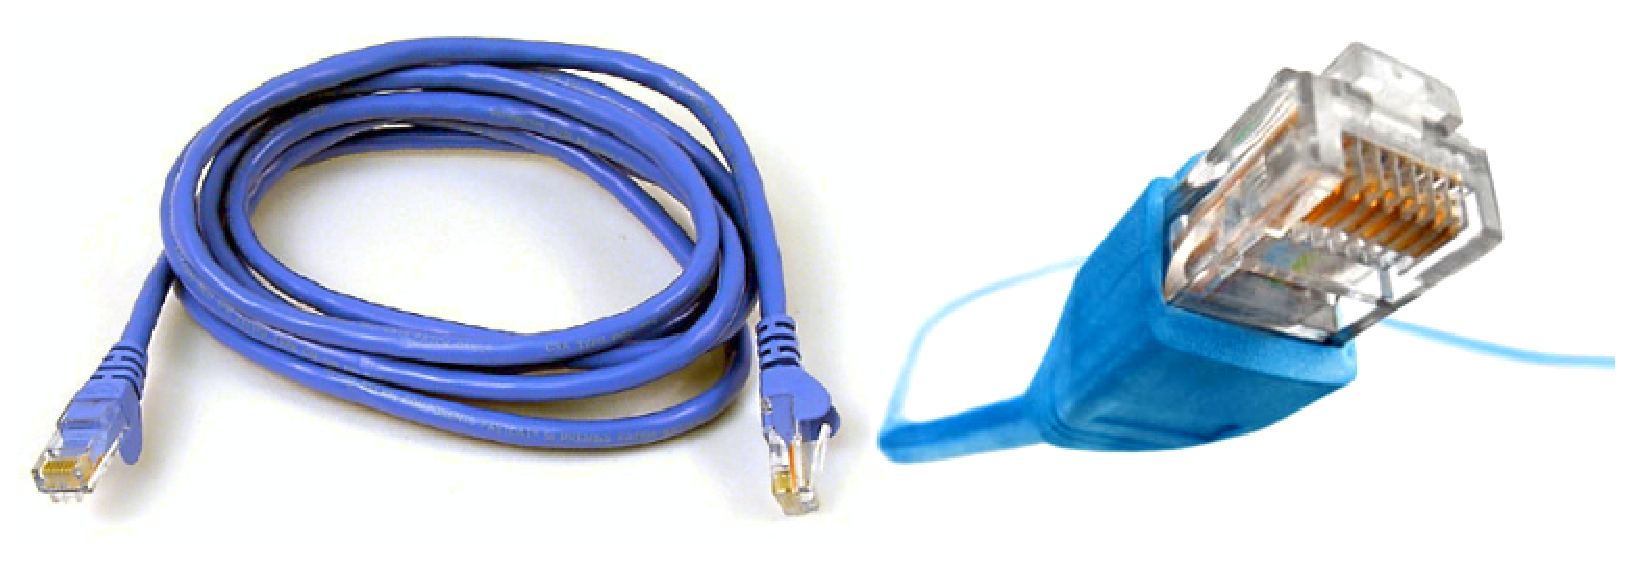
\includegraphics[width=0.9\textwidth]{source/fig/network-cable.eps}}
\caption[Kabel rangkaian Cat-5]{Kabel rangkaian Cat-5}
\label{c2:f3}
\end{figure}

Untuk membuat konfigurasi menggunakan Command Line Interface, pengguna harus mengakses Sistem Terbenam Linux melalui mana-mana kaedah yang telah diterangkan sebelum ini. Ia bermula dengan Login Prompt dimana pengguna harus memasukkan akaun pengguna dan kata laluan yang telah disetkan untuknya.

Sebagai contoh, bagi mengkonfigur IP bagi perkakasan ini, pengguna perlu mengubah fail interfaces yang terdapat di dalam direktori /etc/network/. Berikut adalah contoh arahan yang perlu dilakukan bagi mengubah IP perkakasan ini.
\begin{enumerate}
\item Masukkan akaun pengguna:
{\footnotesize\renewcommand{\baselinestretch}{1.0}
\begin{verbatim}
   Login: root
   Password: ******

\end{verbatim}}

\item Ubah fail /etc/network/interfaces:
{\footnotesize\renewcommand{\baselinestretch}{1.0}
\begin{verbatim}
   root@raingauge:~# nano /etc/network/interfaces
\end{verbatim}}
   aplikasi nano akan dibuka dan berikut adalah contoh kandungan fail tersebut:
{\footnotesize\renewcommand{\baselinestretch}{1.0}
\begin{verbatim}   
   # Used by ifup(8) and ifdown(8). See the interfaces(5) manpage or 
   # /usr/share/doc/ifupdown/examples for more information.
   
   auto lo
   iface lo inet loopback
   
   auto eth0
   #iface eth0 inet dhcp
   iface eth0 inet static
           address 192.168.1.103
           netmask 255.255.255.0
           broadcast 192.168.1.255
           gateway 192.168.1.1
\end{verbatim}}

pengguna harus mengubah baris address, broadcast dan gateway mengikut keperluan mereka.
   
\item Untuk menyimpan konfigurasi yang telah dibuat, kekunci shortcut Ctrl-X digunakan untuk keluar, kemudian kekunci Y untuk Ya jika mahu menyimpan hasil pengubahan dan kekunci enter setelah memastikan nama fail yang ingin diperbaharui.
\end{enumerate}

Untuk mengkonfigur fungsi-fungsi lain, beberapa fail perlu diubah dan inilah kelemahan sistem sedia ada dimana pengguna perlu menghafal nama fail dan arahan-arahan yang perlu diberikan untuk membuat pengubahan fail-fail berkenaan.
       
\subsection{Kajian Terhadap Penyelesaian Semasa}
Hasil kajian yang dilakukan terhadap kaedah penyelesaian semasa bagi menyediakan antaramuka pengguna bergrafik untuk mengautomasikan konfigurasi bagi sistem terbenam Linux, terdapat dua kaedah telah ditemui dalam produk komersil lain bagi mencapai tujuan yang sama:
\begin{enumerate}
\item \textbf{Konfigurasi menggunakan Perisian khusus dari komputer penyelenggara.}

Kaedah menggunakan aplikasi yang ditulis khusus untuk tugas konfigurasi bagi sistem terbenam Linux telah ditemui dalam produk Mikrotik. Aplikasi ini digunakan untuk membuat konfigurasi sistem terbenam Linux yang telah diubahsuai bagi kegunaan komputer berpapan tunggal yang dipanggil RouterBoard keluaran syarikat mereka. Sistem terbenam Linux mereka dipanggil RouterOS yang boleh dipasang dalam pelbagai model RouterBoard keluaran Mikrotik bagi tujuan komunikasi tanpa wayar dan router.

\begin{figure}[!h]
\centering{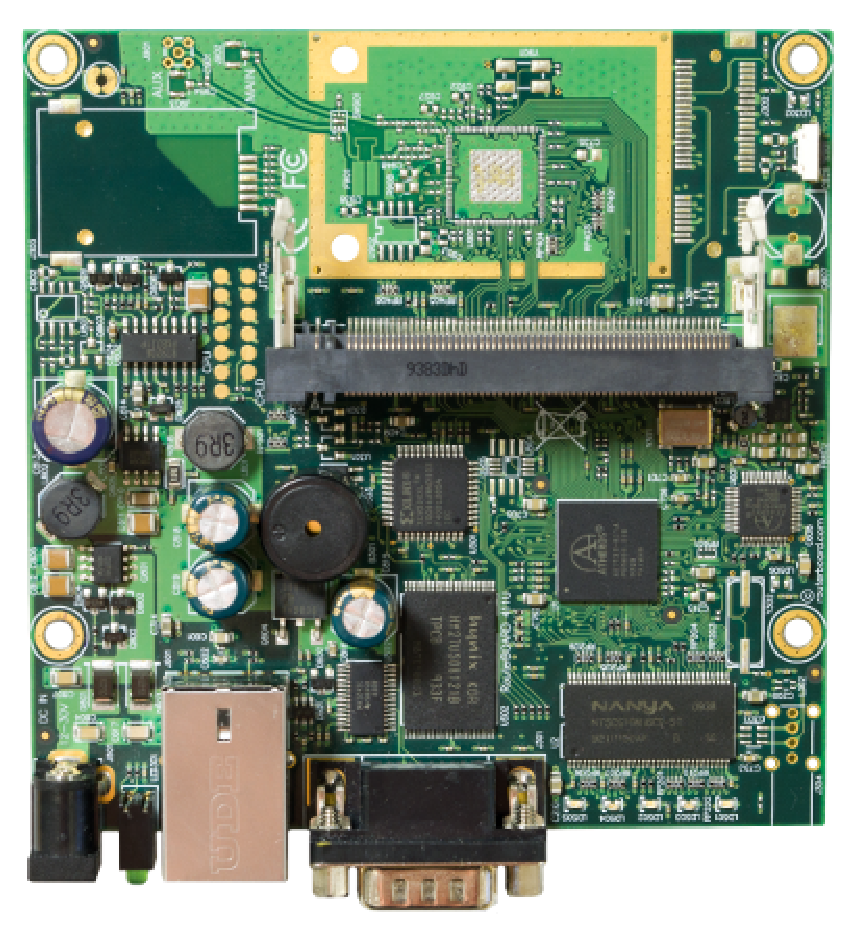
\includegraphics[width=0.9\textwidth]{source/fig/mikrotik-routerboard.eps}}
\caption[Komputer berpapan tunggal RouterBoard keluaran Mikrotik]{Komputer berpapan tunggal RouterBoard keluaran Mikrotik}
\label{c2:f4}
\end{figure}

Aplikasi yang diberi nama Winbox ini boleh dimuat turun secara percuma dari laman web Mikrotik dan boleh terus dilarikan dari mana-mana komputer dengan sistem operasi Windows. Winbox ini boleh digunakan untuk membuat tetapan melalui antaramuka pengguna bergrafik dengan menu yang tersusun dan jadual yang mudah.

\begin{figure}[!h]
\centering{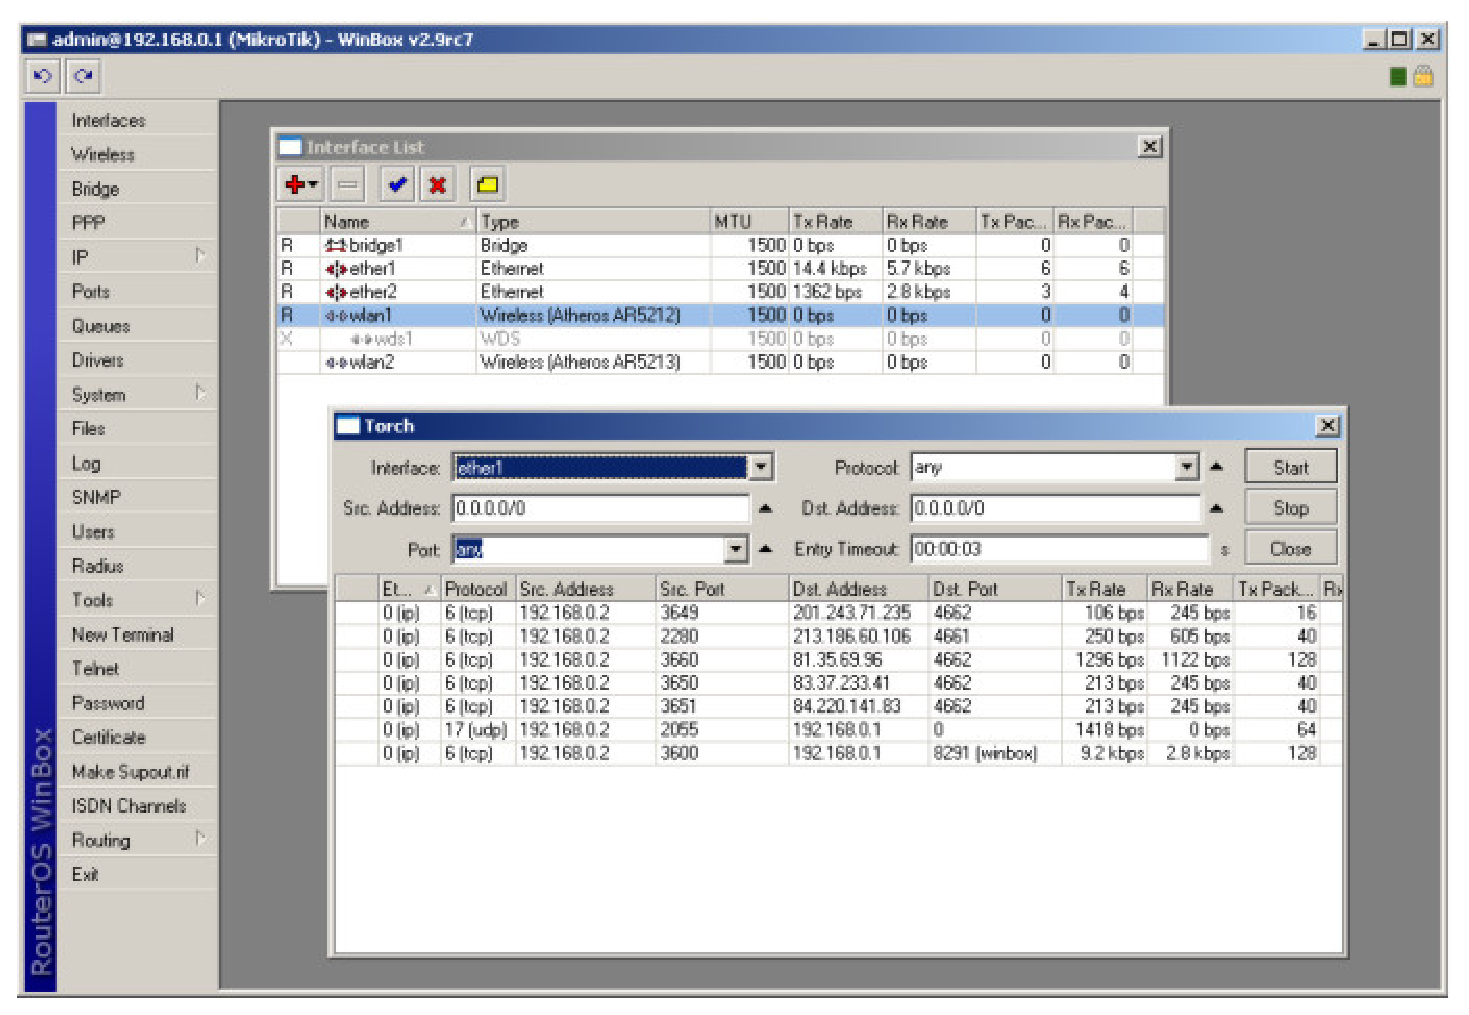
\includegraphics[width=0.9\textwidth]{source/fig/winboxmain.eps}}
\caption[Paparan antaramuka pengguna bergrafik aplikasi Winbox]{Paparan antaramuka pengguna bergrafik aplikasi Winbox}
\label{c2:f5}
\end{figure}

Walau bagaimanapun, kaedah ini tidak meluas dan tertumpu kepada sistem operasi Microsoft Windows kerana aplikasi yang dibina hanya menyokong sistem operasi tersebut. Ini menyukarkan pengguna sistem operasi lain seperti Mac OS X dari Apple, serta sistem operasi berasaskan Linux dan Unix.

\item \textbf{Konfigurasi menggunakan antaramuka web.}

Kaedah konfigurasi menggunakan antaramuka web merupakan kaedah yang agak popular digunakan oleh produk-produk komersial lain. Sistem terbenam Linux yang menggunakan antaramuka web boleh dilihat dalam produk router dan modem seperti modem Streamyx, Unifi dan router popular seperti LinkSYS, D-Link dan Buffalo.

\begin{figure}[!h]
\centering{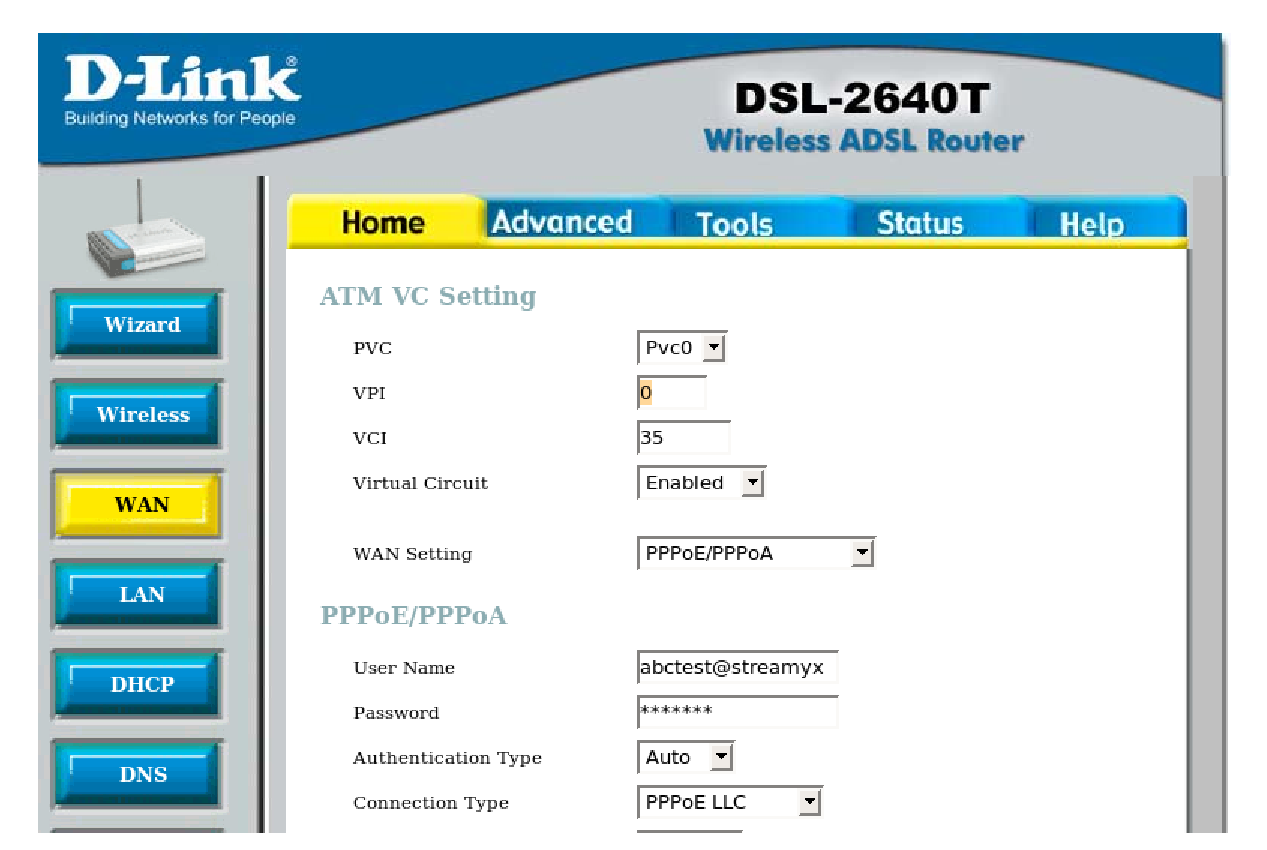
\includegraphics[width=1\textwidth]{source/fig/dlinkshot.eps}}
\caption[Paparan antaramuka web ADSL router D-Link]{Paparan antaramuka web ADSL router D-Link}
\label{c2:f6}
\end{figure}

\end{enumerate}

\section{Kajian Teknologi}
Kajian terhadap teknologi berkaitan sama ada teknologi perisian dan teknologi perkakasan komputer dilakukan demi memastikan kelicinan dan kesesuaiannya dalam penyelesaian masalah yang telah dinyatakan, sumber-sumber sedia ada dalam organisasi, gaya penggunaan aplikasi terkini dan bebas dari isu-isu berkaitan kebolehsokongan terutamanya antara aplikasi-aplikasi yang digunakan berbeza platform, isu berkaitan protokol-protokol perisian, rangkaian dan perkakasan, dan juga ketidakbolehsokongan perkakasan untuk melaksanakan aplikasi-aplikasi yang digunakan semasa pembangunan.

\subsection{Teknologi Perisian}

Dalam pembangunan sistem yang berkait dengan sistem terbenam Linux, pemilihan teknologi perisian yang tepat mestilah dilakukan berpandukan beberapa sebab utama antaranya:
\begin{itemize}
\item Kekangan saiz storan dan sumber perkakasan yang terhad.

\item Jenis pelayan yang akan menyokong kerangka sistem dan jenis bahasa pengaturcaraan yang disokong oleh pelayan tersebut.

\item Kaedah akses pengguna terhadap sistem yang akan dibina.

\end{itemize}

Disebabkan kajian tesis ini melibatkan sistem terbenam Linux yang sedia ada. Pemilihan bahasa pengaturcaraan PHP dan Bash adalah amat bertepatan kerana ianya disokong oleh pelayan Lighttpd yang ringan dan boleh dipasang kedalam sistem ini tanpa menjejaskan prestasi sistem sedia ada. 

\subsubsection{Sistem Terbenam Linux}
Sistem terbenam linux merupakan sebuah sistem terbenam yang dibina berasaskan sistem operasi Linux yang telah dikecilkan saiznya bagi memenuhi keperluan sistem terbenam. Kebanyakan produk untuk kegunaan khusus seperti modem dan router pada hari ini menggunakan sistem terbenam Linux sebagai sistem operasi perkakasan tersebut. Oleh kerana sistem sedia ada iaitu Sistem Tolok Hujan berkeupayaan GPRS ini merupakan sistem terbenam Linux, pembangunan antaramuka bergrafik mestilah bersesuaian dan disokong oleh sistem operasi Linux

\subsubsection{Pelayan Web Lighttpd}
Lighttpd (yang disebut "lighty") adalah sebuah pelayan web bersumber terbuka untuk persekitaran yang kritikal dengan kelajuan bagi produk umum namun mematuhi standard, selamat, dan bolehlentur. Ia pada asalnya ditulis oleh   Jan Kneschke sebagai bukti-konsep bagi permasalahan c10k - bagaimana menangani 10,000 sambungan selari dalam satu pelayan. Pemilihan pelayan ini dilakukan kerana saiznya yang kecil dan ringan tidak akan membebankan dan mengganggu prestasi sistem sedia ada.

\subsubsection{PHP}
PHP: Hypertext Preprocessor adalah bahasa skrip pihak pelayan yang direka untuk pembangunan laman web yang dapat menjana dokumen HTML secara dinamik. PHP dapat digunakan untuk membangunkan sebuah CMS. PHP pada awalnya ditulis oleh Rasmus Lerdorf pada tahun 1995. Pada ketika itu, ia diberi nama Form Interpreted (FI), yang merupakan sekumpulan skrip yang digunakan untuk mengolah data dan formula dari web. Rasmus kemudiannya telah membebaskan kod sumber tersebut kepada umum dan menamakannya PHP/FI. Dengan pembebasan kod sumber ini menjadi sumber terbuka, ia menarik lebih ramai pembangun dan pengaturcara untuk sama-sama mengembangkan PHP. Bahasa pengaturcaraan ini dipilih dalam pembangunan antaramuka bergrafik sistem terbenam Linux kerana kebolehlenturannya dan kemampuannya membina antaramuka web yang dinamik.

\subsubsection{Bash}
Bash ialah Unix shell yang ditulis oleh Brian Fox untuk Projek GNU sebagai pengganti kepada Bourne Shell (sh). Diterbitkan pada 1989, ia telah diedarkan dengan meluas sebagai shell kepada sistem operasi GNU dan sebagai default shell dalam Linux, Mac OSX dan Darwin. Ia kemudiannya telah diportkan untuk Microsoft Windows dan diedarkan bersama Cygwin dan MinGW, kepada DOS oleh projek DJGPP dan kepada Novell Netware.

Bash ialah pemproses perintah yang lazimnya dilarikan dalam tetingkap teks, membenarkan pengguna menaip perintah yang akan melakukan sesuatu tugas. Bash juga boleh membaca perintah-perintah yang disimpan di dalam fail yang dipanggil skrip. Seperti Unix shell yang lain, ia memahami wildcarding, piping, dokumen here, pengganti perintah, pembolehubah, dan struktur kawalan untuk ujian keadaan dan iterasi. Katakunci, sintaks, dan segala ciri-ciri asas bahasa arahannya telah ditiru dari sh. Manakala ciri-ciri lain seperti history, telah ditiru dari csh dan ksh. Bash ialah POSIX shell tetapi dengan beberapa \textit{extensions}.

Namanya merupakan akronim, yang mempunyai maksud tersirat dan penuh makna. Sebagai akronim, ia bermaksud Bourne-again Shell, yang merujuk kepada objektifnya sebagai pengganti kepada Bourne shell. Sebagai maksud tersirat pula, ia memberi objektif kepada prosa yang berbunyi seperti 'born again' dalam bahasa Inggeris yang bermaksud kelahiran semula. Nama ini juga dikira penuh makna seperti apa yang boleh dilakukannya, 'bashing together' yang bermaksud mencampur aduk semua ciri-ciri sh, csh dan ksh kedalamnya. 

\subsubsection{CGI}
CGI ialah singkatan kepada Common Gateway Interface yang merupakan protokol piawai untuk mengantaramuka perisian aplikasi luaran dengan pelayan maklumat yang biasanya pelayan web. Tugas bagi pelayan maklumat ini adalah untuk memberi respon kepada permintaan pelanggan dengan mengembalikan output. Contohnya, bagi pelayan web yang memberi respon kepada pelanggannya iaitu pelayar web.

Protokol ini boleh digunakan untuk menjalankan Shell Script yang berfungsi untuk mengautomasikan konfigurasi dengan mengambil input dari permintaan pelayar web. Terdapat banyak program yang boleh dilaksanakan oleh Shell Script serta dapat digunakan dengan adanya teknologi CGI ini. Dalam projek pembangunan antaramuka bergrafik ini, FastCGI dipasang dan digunakan bersama pelayan web Lighttpd bagi menyokong bahasa skrip PHP untuk menjana output HTML.

\subsubsection{HTML}
HTML adalah singkatan daripada Hyper Text Markup Language. Ia adalah bahasa yang difahami oleh pelayar web bagi memaparkan antaramuka pengguna bergrafik web. Dengan bahasa ini, pelayar web dapat membezakan elemen-elemen dari maklumat berasaskan teks di dalam dokumen HTML kepada teks, pautan, jadual, perenggan, senarai, dan sebagainya. Ia juga menerangkan bahawa teks tersebut juga beserta dengan borang interaktif, imej terbenam dan objek-objek lain. HTML ditulis dalam bentuk tag yang dirangkumi di dalam braket sesiku (angle bracket). Dari segi konvensyen, data dalam format HTML menggunakan extension .html atau .htm. Bahasa HTML sangat penting dalam penghasilan laman web. Ianya akan digunakan untuk membentuk antaramuka pengguna bergrafik bagi projek ini.

\subsubsection{JavaScript}
JavaScript merupakan bahasa scripting yang biasa digunakan untuk pembangunan web dipihak pelanggan (client-side). Ia berasal dari dialek piawai ECMAScript. JavaScript telah dipengaruhi oleh banyak bahasa pengaturcaraan dan direka agar kelihatan seperti Java, tetapi agak mudah untuk dikendalikan oleh mereka yang bukan pengaturcara. Ia biasanya digunakan untuk menjadikan laman web lebih bertindakbalas dan kelihatan hidup. Dalam projek ini, teknologi JavaScript digunakan untuk membantu menghasilkan antaramuka pengguna berasakan web yang lebih interaktif.

\subsubsection{CSS}
Cascading Style Sheet atau CSS adalah teknologi yang membolehkan sesebuah laman web mempunyai format rekaletak yang seragam. Ia merupakan bahasa stylesheet yang digunakan untuk menerangkan bentuk persembahan sesuatu dokumen yang ditulis menggunakan bahasa markup seperti HTML dan XHTML. Dengan menggunakan teknologi CSS dalam penghasilan laman web, pengguna akan mudah memahami antaramuka web tersebut kerana bentuk, tema warna dan lokasi yang seragam.

\subsection{Teknologi Perkakasan Komputer}
Terdapat beberapa perkakasan utama yang digunakan dalam pembangunan projek ini. Perkakasan ini terdiri daripada Single Board Computer (SBC) atau Komputer berpapan tunggal, Komputer peribadi, sambungan rangkaian atau sambungan serial RS-232.

\subsubsection{\textit{Single Board Computer}}

\begin{figure}[!h]
\centering{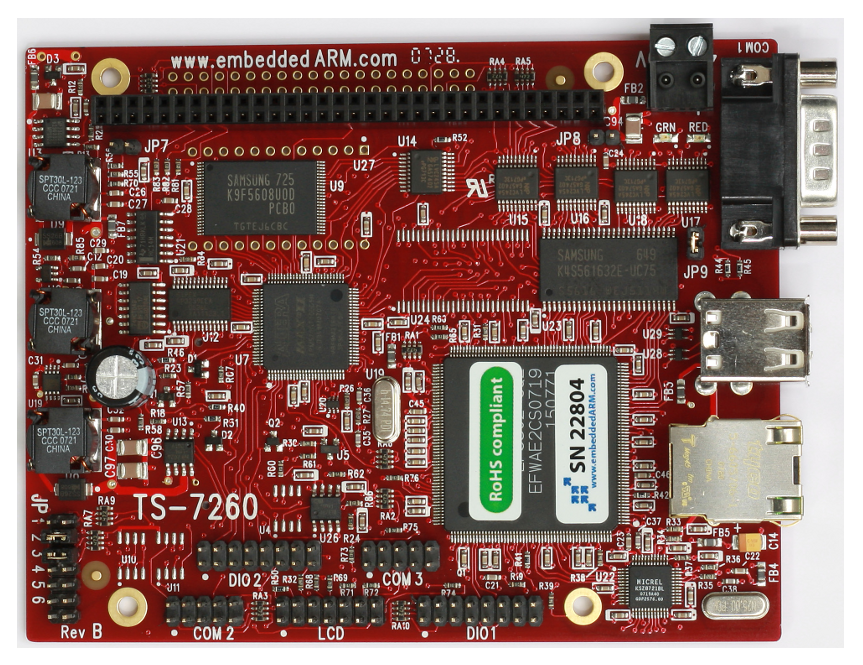
\includegraphics[width=1\textwidth]{source/fig/ts7260.eps}}
\caption[Single Board Computer (SBC) atau Komputer Berpapan Tunggal]{Single Board Computer (SBC) atau Komputer Berpapan Tunggal}
\label{c2:f7}
\end{figure}

\newpage

Single Board Computer (SBC) atau Komputer Berpapan Tunggal merupakan sebuah perkakasan yang mempunyai keupayaan sebuah komputer dengan sumber yang dikurangkan pada kadar paling minimum. Ia biasanya dibekalkan bersama sistem operasi terbenam Linux yang terdapat dipasaran. Sistem Terbenam Linux yang digunakan dalam Tolok Hujan berkeupayaan GPRS ini merupakan sistem operasi berteraskan kernel Linux dari distro Debian-ARM. Tolok Hujan ini dibina menggunakan komputer berpapan tunggal model TS-7260 keluaran Technologic Systems. 

\subsubsection{Komputer Peribadi atau Laptop}
Komputer peribadi atau Laptop digunakan bagi mengakses sistem terbenam Linux melalui hubungan SSH dan Protokol HTTP. Oleh kerana sistem terbenam Linux yang digunakan dalam projek ini merupakan sistem tanpa kepala dan mempunyai sumber serta ruang storan yang kecil, komputer peribadi juga digunakan untuk membangunkan antaramuka bergrafik bagi sistem ini.

\subsubsection{Sambungan Rangkaian bagi Sistem Tanpa Kepala}
Sambungan rangkaian dari komputer peribadi disambungkan kepada port rangkaian SBC untuk mengakses antaramuka CLI dan antaramuka bergrafik sistem terbenam Linux ini. Ini dilakukan dengan menggunakan kabel rangkaian Cat-5 atau Cat-6 yang dipasang terus dari komputer peribadi kepada SBC.

\section{Kesimpulan}
Kewujudan pelbagai inovasi kejuruteraan perisian dan perkakasan pada hari ini merupakan suatu perkembangan yang sihat bagi memenuhi kepelbagaian permintaan terhadap aplikasi atau penyelesaian yang bijak dan kompetitif dalam industri. Kepelbagaian dalam senarai produk yang boleh dipilih bagi tujuan khusus membolehkan kita membuat pilihan yang bertepatan dan bersesuaian dengan kehendak, kos dan kekangan sistem. Kepentingan untuk membuat kajian dalam pemilihan produk perisian dan perkakasan yang tepat adalah mandatori bagi mendapatkan hasil yang memenuhi kehendak dan matlamat projek.
